

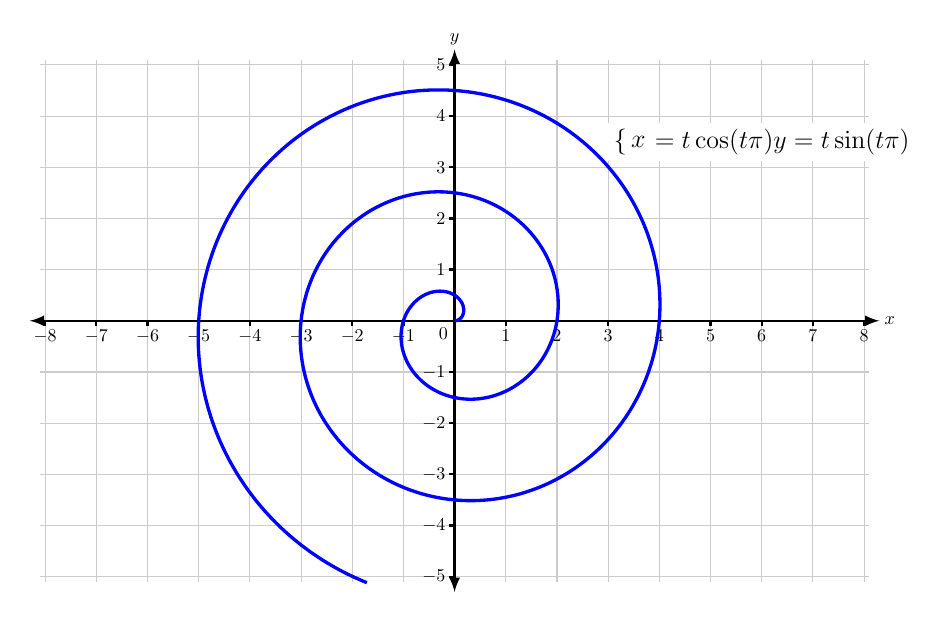
\begin{tikzpicture}[thick,scale=0.65, every node/.style={scale=0.65}]
  \def \minx {-8}
  \def \maxx {8}
  \def \miny {-5}
  \def \maxy {5}

  \draw[thin,black!20] (\minx-0.1,\miny-0.1) grid (\maxx+0.1,\maxy+0.1);

  \draw[thick, latex-latex] (\minx-0.3,0)--(\maxx+0.3,0);
  \draw[thick, latex-latex] (0,\miny-0.3)--(0,\maxy+0.3);
  \node at (\maxx+0.5,0) {$x$};
  \node at (0,\maxy+0.5) {$y$};

  \foreach \x in {\minx,...,-1}{
    \draw (\x,0)--(\x,-0.1);
    \node[below,black] at (\x,-0.05) {$\x$};
  }
  \foreach \x in {1,...,\maxx}{
    \draw (\x,0)--(\x,-0.1);
    \node[below,black] at (\x,-0.05) {$\x$};
  }
  \foreach \y in {\miny,...,-1}{
    \draw (0,\y)--(-0.1,\y);
    \node[left,black] at (-0.05,\y) {$\y$};
  }
  \foreach \y in {1,...,\maxy}{
    \draw (0,\y)--(-0.1,\y);
    \node[left,black] at (-0.05,\y) {$\y$};
  }
  \node[below left,black] at (0,0) {$0$};

  \draw[
    very thick,
    domain=0:5.4,
    variable=\t,
    smooth,
    samples=300,
    blue]
    plot ({\t*cos(\t*3.1415 r)},{\t*sin(\t*3.1415 r)});

  \node at (6,3.5) [fill=white]
  {
      \Large
      $
      \begin{cases}
        x = t \cos(t\pi) \\
        y = t \sin(t\pi)
      \end{cases}
      $
  };
\end{tikzpicture}
